\documentclass[a4paper,11pt,dvipdfmx]{ujarticle}
\usepackage{graphicx}
\usepackage{url}
\input{layout}

\title{日本におけるデジタル化の状況}
\author{G584942025 森 冠太}

\begin{document}

\maketitle 

 \section{デジタル競争力ランキング}

国際経営開発研究所(IMD)の調査\cite{imd}によると、日本のデジタル競争力のランキングは図\ref{fig:ランキング}に示すよ
うに、調査対象の64カ国中、総合で28位、知識分野で25位となっている。
\begin{figure}[htbp]
    \centering
    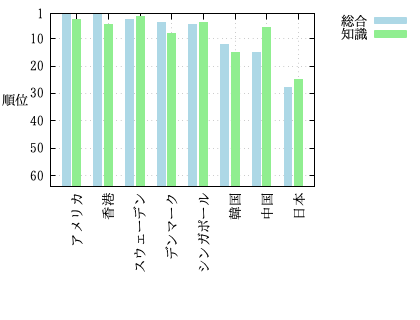
\includegraphics[width=0.7\linewidth]{fig31.png}
    \caption{デジタル競争力ランキング(64カ国中)}\label{fig:ランキング}
\end{figure}

 
\newpage
\maketitle
 
 \section{ブロードバンドの整備状況}

OECDによるブロードバンド回線の普及に関する調査\cite{oecd}によると、表\ref{tbl:加入者数}に示すように、日本における 100人あたりのモバイルブロードバンドの加入者数は190.5で、第1位になっている。2位はエストニア
で、3位米国と続く。

\begin{table}[htbp]
    \centering
    \caption{:モバイルブロードバンドの加入者数(100人あたり)}
    \label{tbl:加入者数}
    
    \begin{tabular}{|c|l|r|}\hline
        順位 & 国名 & 加入者数 \\
        \hline
        1位 & 日本 & 190.5 \\
        \hline
        2位 & エストニア & 179.9 \\
        \hline
        3位 & 米国 & 169.0 \\
        \hline
        4位 & フィンランド & 157.0 \\
        \hline
        5位 & デンマーク & 141.7 \\
        \hline
        6位 & ラトピア & 141.6 \\
        \hline 
        7位 & イスラエル & 139.9 \\
        \hline
        8位 & オランダ & 133.7 \\
        \hline
        9位 & ポーランド & 131.3 \\
        \hline
        10位 & スウェーデン & 127.2 \\
        \hline
    \end{tabular}
\end{table}

\maketitle
 \section{考察}

\begin{itemize}
    \item 日本はデジタル競争力ランキングで28位と、先進国の中では低い位置にあるのは知識があっても活用する力が低いからだと考えられる。
    \item ブロードバンドの整備状況は良好で、モバイルブロードバンドの加入者数は世界第1位であるのはインフラ整備に優れているからだと考えられる。
    \item 以上のことから、日本はインフラ整備には強いが、活用力が弱いため、デジタル競争力が低いと考える。
\end{itemize}
 
\bibliographystyle{junsrt}
\bibliography{exercise.bib}

\end{document}